\documentclass[tikz]{standalone}
\usepackage{pgfplots}\pgfplotsset{compat=1.17}
\begin{document}
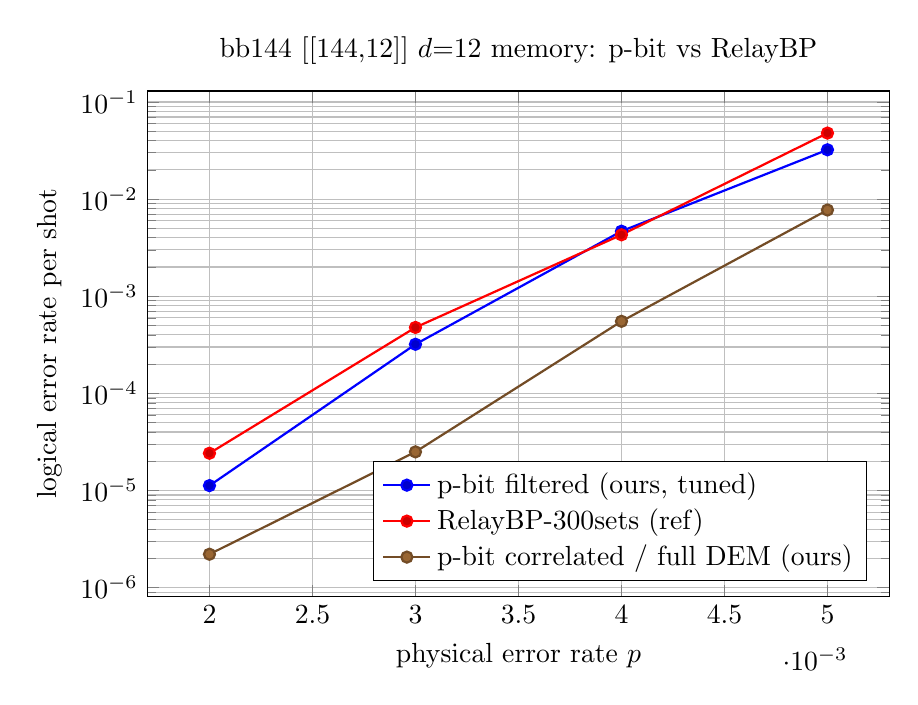
\begin{tikzpicture}
\begin{semilogyaxis}[
  width=11cm,height=8cm,xlabel={physical error rate $p$},
  ylabel={logical error rate per shot},
  title={bb144 [[144,12]] $d{=}12$ memory: p-bit vs RelayBP},
  grid=both,legend pos=south east,legend cell align=left]
\addplot+[thick,mark=*] coordinates {(0.002,1.1230e-05) (0.003,3.2031e-04) (0.004,4.6719e-03) (0.005,3.2188e-02)};
\addlegendentry{p-bit filtered (ours, tuned)}
\addplot+[thick,mark=*] coordinates {(0.002,2.4193e-05) (0.003,4.7742e-04) (0.004,4.2910e-03) (0.005,4.7836e-02)};
\addlegendentry{RelayBP-300sets (ref)}
\addplot+[thick,mark=*] coordinates {(0.002,2.2088e-06) (0.003,2.5000e-05) (0.004,5.5208e-04) (0.005,7.7222e-03)};
\addlegendentry{p-bit correlated / full DEM (ours)}
\end{semilogyaxis}
\end{tikzpicture}
\end{document}
